%Data_to_Computer
We now have voltage data coming from our Arduino into the computer serial
port, and we can see that data with the Arduino serial port monitors. But
suppose we want to analyze our data in another program. How would we get the
data into Excel or LoggerPro, or SPSS or even our beloved Python that we
learned to use in PH150?

There are lots of ways to do this, but an easy way is to use our Python
skills and write a simple code using the Python serial port library. That is
what we are going to do in this lab.

\section{How to get Python}

But wait, you might say, I didn't use snakes in PH150. What are you even
talking about? Or maybe you got rid of Python because you never thought you
would use it again. Whatever the case, Python is another way to make
computer code like our Arduino app. Only, this code is designed to work on
our computer, itself. This is just what we want for getting the data ready
for analysis on our computer. If you already have Python, that is fine, you
could skip ahead. If you don't, the next steps show how to get Python on
your computer and how to get the Python serial library so you have the
commands to read the serial port. Our physics department uses two different
distributions of Python. Canopy, and Anaconda. Canopy is a little bit more
\textquotedblleft civilized\textquotedblright\ with more dialogue boxes and
little command line work. Anaconda is a little bit more \textquotedblleft
linux-like\textquotedblright\ with more command line work. But both work
fine. Instructions for getting both are in the sections below.

\subsection{Getting Anaconda Python}

The Anaconda distribution of Python is designed for scientific work (so it
has most of the science libraries of functions already installed) It can be
found at https://www.continuum.io/downloads. There is an install link for
Windows, Mac, and Linux. Choose the one for your operating system\footnote{%
If you have a Linux computer, it is likely that you will want to actually
see if Anaconda is in your distribution's repository. If you are not a Linux
user, you have no idea what that means and can ignore it.}.

When you click on a link, it is likely a dialog box will come up telling you
that you are downloading something. In windows it looks like this \begin{figure}[h!]
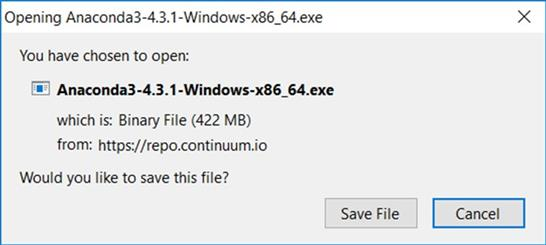
\includegraphics[width=4.5939in,height=2.0721in]{PH4CAU23}
\end{figure}

Choose \textquotedblleft Save File\textquotedblright\ and when the file is
downloaded open it to start the installation. You should see something like
this: \begin{figure}[h!]
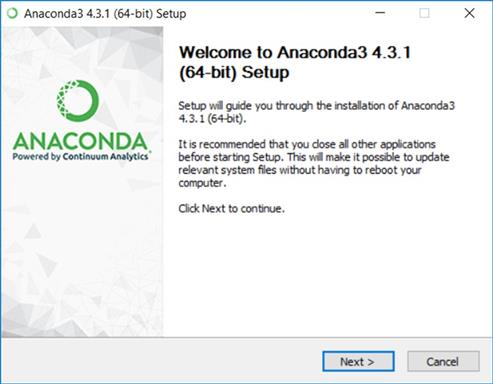
\includegraphics[width=4.1502in,height=3.2361in]{PH4CAU24}
\end{figure}

Choose \textquotedblleft Next\textquotedblright\ and follow the installation
instructions. If all goes well, you should have a new set of apps. Here is
what mine looked like on my Windows 10 computer. \begin{figure}[h!]
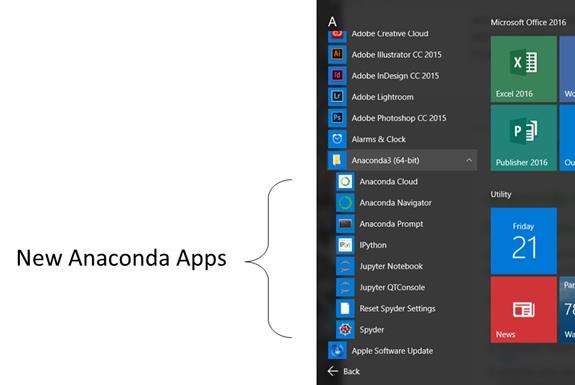
\includegraphics[width=4.8369in,height=%
3.2448in]{PH4CAU25}
\end{figure}

The list of the apps has an app called Spyder. Let's launch it to see what
it does.\begin{figure}[h!]
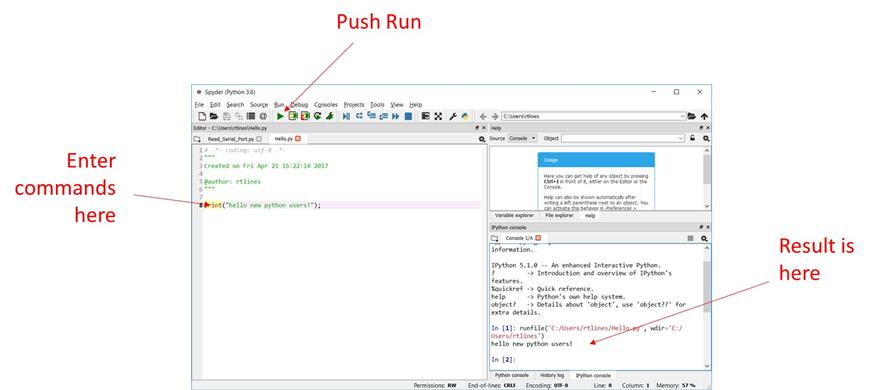
\includegraphics[width=5.655in,height=2.4898in]{PH4CAU26}
\end{figure}

What we get is something like the Arduino program that we have been using to
write Arduino sketches. Spyder is a place to write and run Python commands.
Only this time there is no checking and uploading the code, because the
Python code will run on our computer, not on an Arduino.

In the figure above, the command just says to print \textquotedblleft hello
new python users!\textquotedblright\ and that is all. When it runs, it
prints our message on the small window to the right. But of course Python
can do much more than print silly messages in little windows. We will have
our Python system read a serial port and save our data to a file. But we
need an additional piece of Python to do this. We need functions that can
handle serial ports. These functions are already written by someone, and put
together in a package called a \textquotedblleft library.\textquotedblright\
But this library isn't included in what we have downloaded. So we need to
fix this next.

\subsection{Getting the PySerial library for Anaconda.}

Now that we have Python, we need to update it with the PySerial library so
that we can read our data from the computer serial port. If you have
installed the Anaconda package as your Python distribution, follow along
here. If you have Canopy, see the instructions below (section \ref{Canopy}).
If you have a different distribution entirely, ask your instructor for help.

We will use the Anaconda prompt to get the PySerial library. The Anaconda
prompt is an app that let's us modify the Python libraries that we have
installed. The Anaconda prompt is found in the list of apps that were
installed in Anaconda. If you are using Windows, you might find it in your
app list like this.

\begin{figure}[h!]
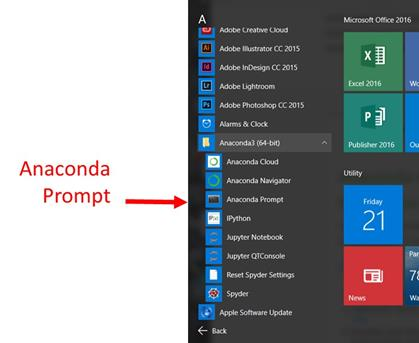
\includegraphics[width=3.5293in,height=2.8928in]{PH4CAU27}
\end{figure}

Once you launch the Anaconda prompt it just looks like a big black box. 
\begin{figure}[h!]
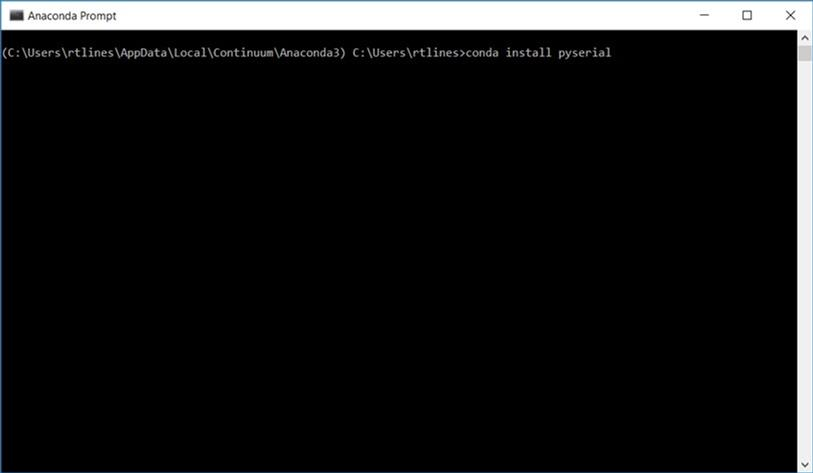
\includegraphics[width=5.2831in,height=3.0796in]{PH4CAU28}
\end{figure}We can type commands in that box
that will modify the Anaconda Python programs that we installed. In our case
we want to type in the command \texttt{conda install pyserial}.

\begin{figure}[h!]
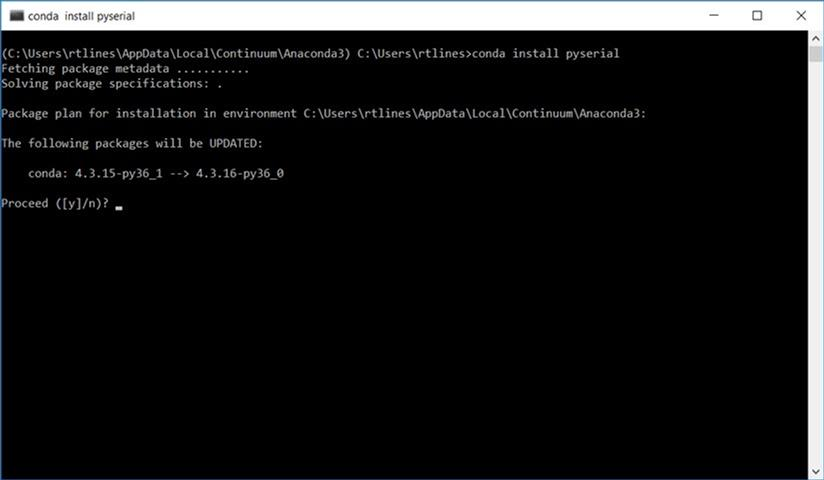
\includegraphics[width=5.1664in,height=3.0156in]{PH4CAU29}
\end{figure}

Notice that the Anaconda prompt app responds to our command. What it
responds will depend on your computer and your Python distribution. You need
a network connection to install new libraries, so if you get an error, you
may just not be connected to a network.

\begin{figure}[h!]
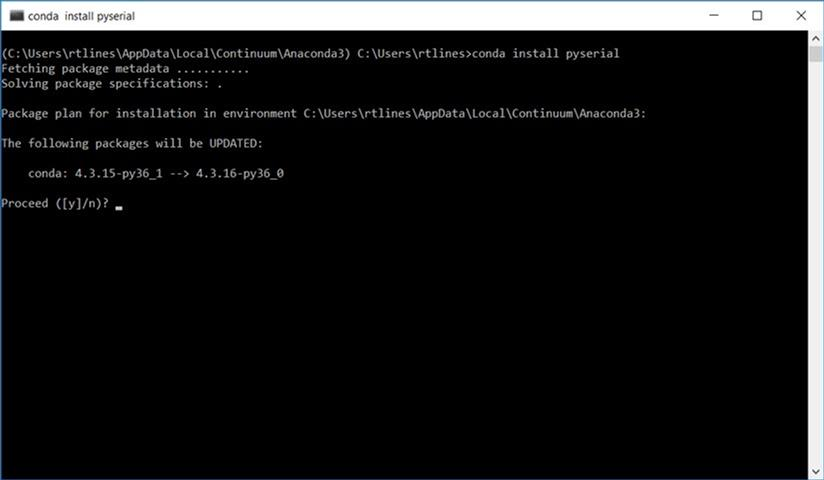
\includegraphics[width=4.2851in,height=2.501in]{PH4CAU2A}
\end{figure}If you already have PySerial
installed, you will be told so, or asked if you wish to update it if an
update is available. If you don't have PySerial, it will ask you if you want
to install it. Answer \textquotedblleft yes\textquotedblright\ and PySerial
will be installed. If any error messages are generated, ask for help from
your instructor. Hopefully you will see a happy end result like this \begin{figure}[h!]
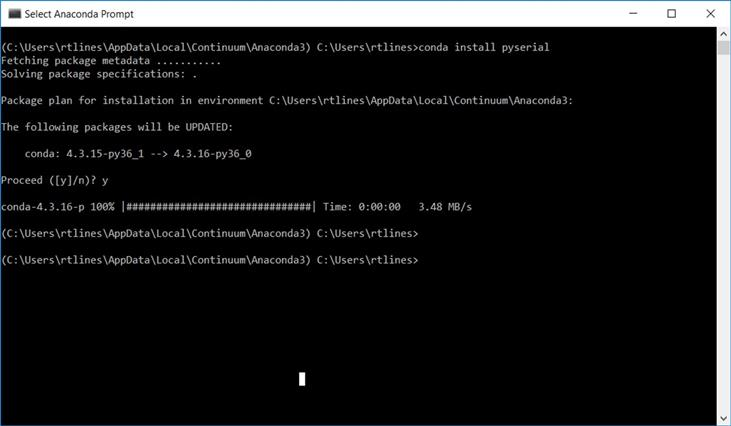
\includegraphics[width=6.1445in,height=3.589in]{PH4CAU2B}
\end{figure}%
and you will be all ready to start writing code to get data from the serial
port.

\section{Getting Canopy Python}

If you choose the Canopy system, follow these instructions. You may already
have the Canopy distribution of Python. If so skip down to adding PySerial
in the next section.

Canopy is a little more polished in it's setup. And it works well. So let's
see how to install this version of Python and enhance it with the Pyserial
library. We will start at the Canopy home site
https://www.enthought.com/products/canopy/. Partway down the page there is a
blue \textquotedblleft Download Canopy\textquotedblright\ button.

\begin{figure}[h!]

\includegraphics[width=3.0219in,height=1.7988in]{PH4CAU2C}
\end{figure}This will take you to the
download page where you can choose the version for your operating system.
When you click the proper download link, it will ask you for some
information. \begin{figure}[h!]
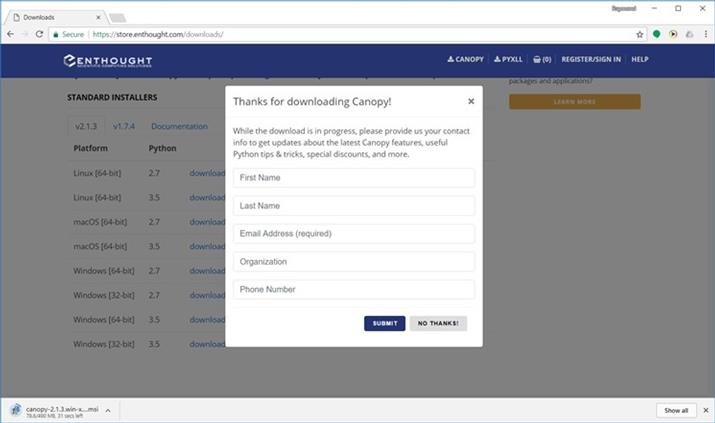
\includegraphics[width=6.0164in,height=3.5674in]{PH4CAU2D}
\end{figure}

Once the download completes, install Canopy. When you run the program, you
will see something like this\begin{figure}[h!]
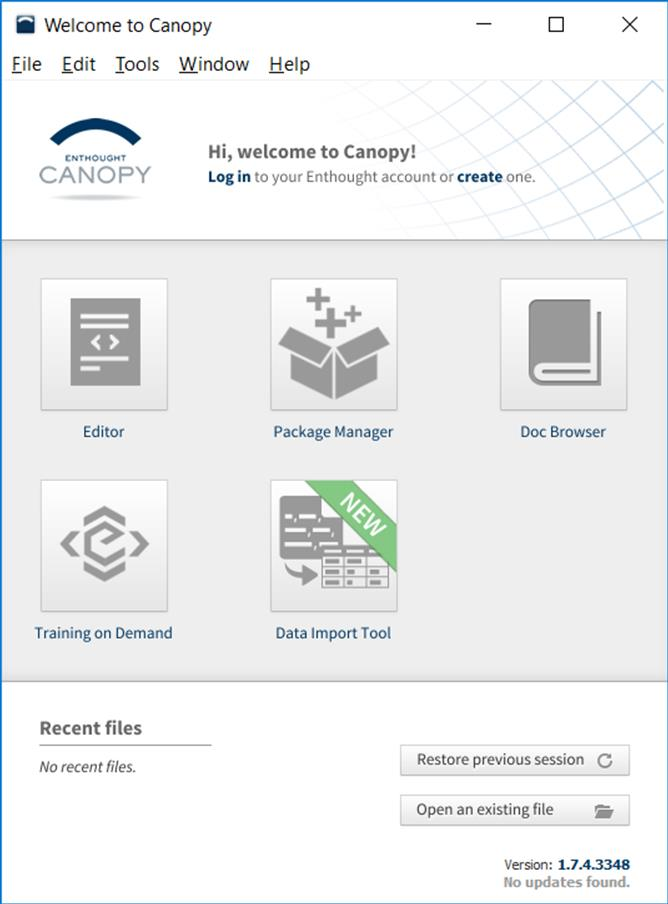
\includegraphics[width=1.983in,height=2.6775in]{PH4CAU2E}
\end{figure}

The editor lets us write Python programs. If you choose this you get a
window like our Arduino program. \begin{figure}[h!]
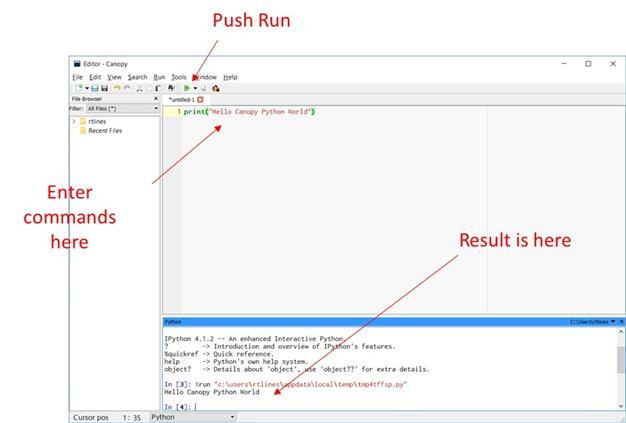
\includegraphics[width=5.2641in,height=3.563in]{PH4CAU2F}
\end{figure}The editor is a place to write
and run Python commands very like our Arduino softare. Only, this time there
is no checking and uploading the code, because the Python code will run on
our computer, not on an Arduino.

In the figure above, the command just says to print \textquotedblleft Hello
Canopy Python World\textquotedblright\ and that is all. When it runs, it
prints our message on the small window at the bottom of the Editor window.
But of course Python can do much more than print silly messages in little
windows. We will have our Python system read a serial port and save our data
to a file. But we need an additional piece of Python to do this. We need
functions that can handle serial ports. These functions are already written
by someone, and put together in a package called a \textquotedblleft
library.\textquotedblright\ But this library isn't included in what we have
downloaded, so we need to fix this next.

\subsection{Getting the PySerial library for Canopy\label{Canopy}}

Now that we have Python, we need to update it with the PySerial library so
that we can read our data from the computer serial port. If we go back to
the Canopy main window we will see a \textquotedblleft Package
Manager.\textquotedblright\ The Package manager lets us add new parts of
Python, and that is just what we want to do. Choose the Package Manager and
in its search box type in \textquotedblleft pyserial.\textquotedblright 
\begin{figure}[h!]
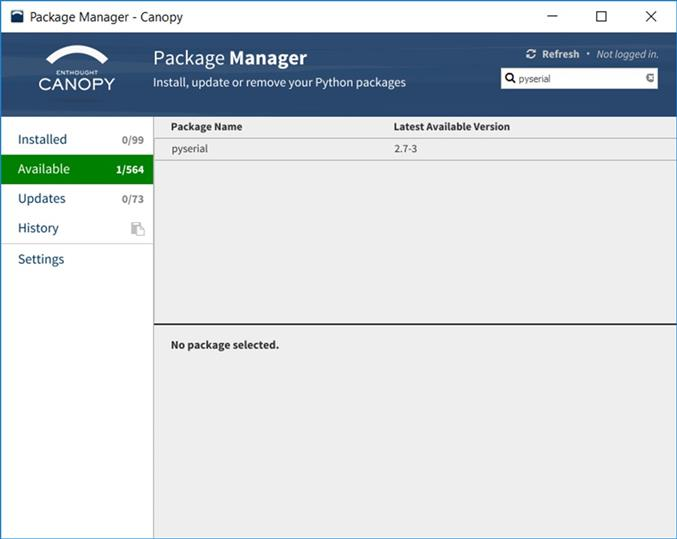
\includegraphics[width=3.9302in,height=3.1328in]{PH4CAU2G}
\end{figure}

It won't initially find pyserial because it is not yet installed and we are,
by default, looking at what is installed. But choose the \textquotedblleft
Available\textquotedblright\ tab. Now we see pyserial in the package list.
Select Pyserial\begin{figure}[h!]
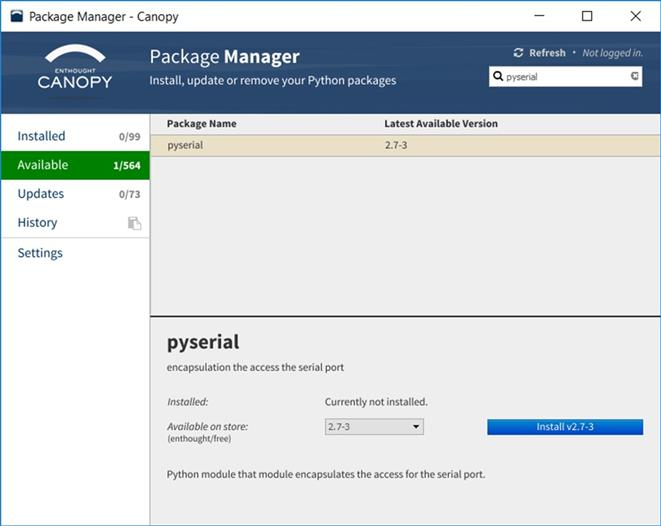
\includegraphics[width=4.0588in,height=3.233in]{PH4CAV2H}
\end{figure}and choose the install button
that appears. If all goes well, you will see a red \textquotedblleft
uninstall\textquotedblright\ button appear.\begin{figure}[h!]
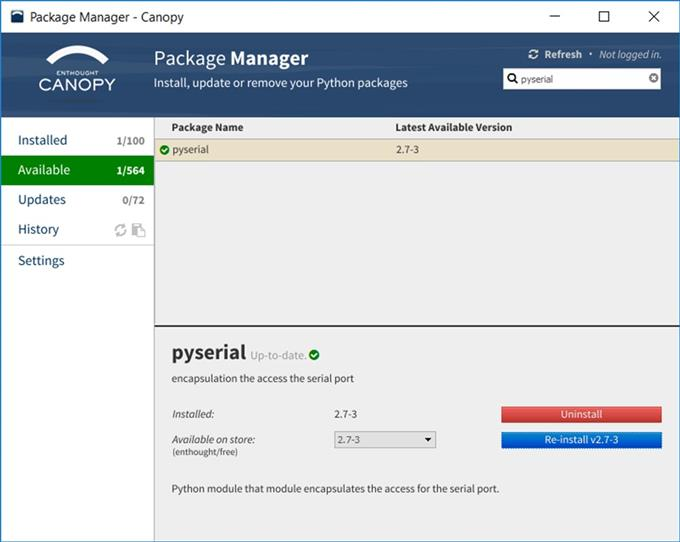
\includegraphics[width=4.4849in,height=3.5786in]{PH4CAV2I}
\end{figure}

Now we can go back to the editor and write our code to read the serial port. 
\begin{figure}[h!]
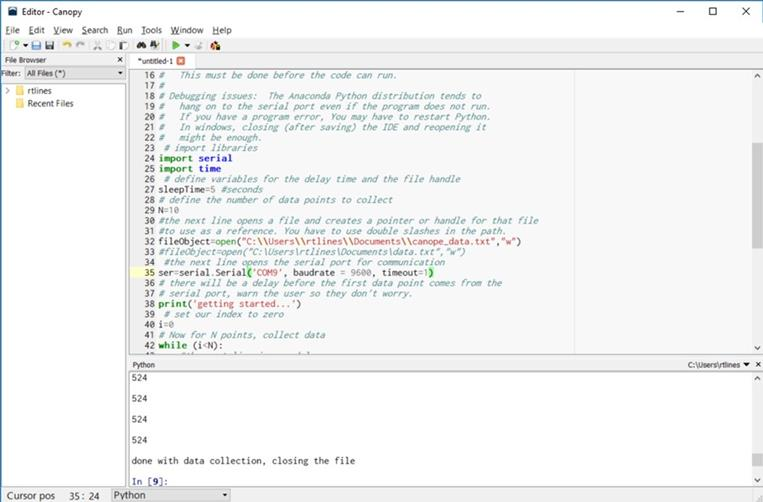
\includegraphics[width=5.227in,height=3.4442in]{PH4CAV2J}
\end{figure}

\section{Getting data from the Arduino}

It might help to know how a serial port works. The serial port in the
computer takes in data from the serial cable. It stores the data in a
temporary place in memory called a \emph{buffer}. Whatever data comes into
the port goes into that memory location. \begin{figure}[h!]
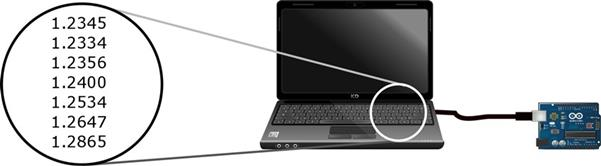
\includegraphics[width=4.5826in,height=1.2791in]{PH4CAV2K}
\end{figure}

Suppose that we set up our Arduino to send data to the port. The Arduino
sends data every few milliseconds. But, suppose we only want data every few
seconds. We only want some of the data that the Arduino has sent. \begin{figure}[h!]
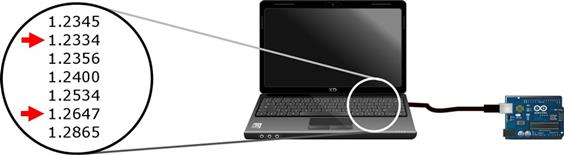
\includegraphics[width=4.7444in,height=1.3188in]{PH4CAV2L}
\end{figure}%
The computer has placed every data point sent by the Arduino into it's
buffer, and the buffer must be read in sequence. You can't skip data values.
But this is just what we want to do, skip some data values and take a value
every few seconds. A way to do this is to continuously read in data, but
only store it every few seconds. We will use this technique in the code that
follows.

Just for fun, let's think of an actual data collection. Suppose we want to
measure a voltage from our Arduino, but we want to measure it many times,
each time five seconds apart. This way we are looking at how the voltage
changes over time. We might want $10$ total measurements.

You might be an expert Python programmer, and if so you can probably see how
to write this code. If so, go ahead and do so. But if not, let me introduce
some of the Python code elements we will need, and then give an example code.

The first new code piece is making files for our data. We create a file with
a line like this (see the actual code below):%
\begin{equation*}
\begin{tabular}{l}
\texttt{fileObject=open("C:$\backslash$$\backslash$%
Users$\backslash$$\backslash$rtlines$\backslash$$\backslash$Documents$\backslash$%
$\backslash$data.txt","w")}%
\end{tabular}%
\end{equation*}%
The \textquotedblleft fileObject\textquotedblright\ is a variable that
contains all the file information like the path and file name. It is way
easier to type than to include all that information each time we use a file.
So we will use fileObject variables. In the code below I named the
fileObject variable \textquotedblleft dataFile.\textquotedblright\ Of
course, you will have to choose your own path where you will place the data
file (you can't use mine, because you don't have my computer!) and you will
need to choose your own file name. Notice the weird double slashes
\textquotedblleft $\backslash$$\backslash$%
.\textquotedblright\ These are a Python thing and you need to write the path
this way.

The other new code piece is dealing with serial ports. Like with our Arduino
code, we have to set up the serial port. We do that with the line like the
this (also see the actual code below).

\begin{equation*}
\begin{tabular}{l}
\texttt{ser=serial.Serial('COM6', baudrate = 9600, timeout=1))}%
\end{tabular}%
\end{equation*}%
Note that when I was using this code my Arduino was in COM6. But that might
not be true for you. Use the Arduino app to find out where your Arduino is
connected. \begin{figure}[h!]
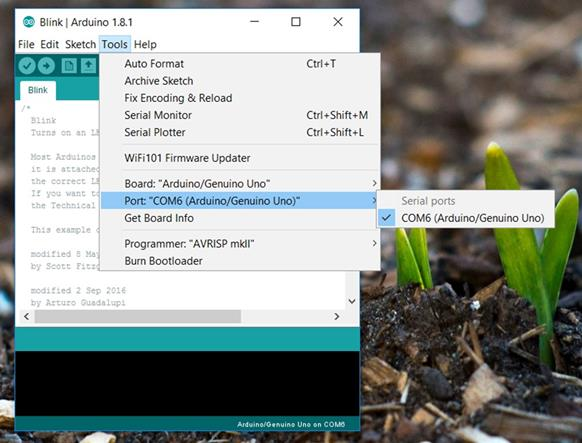
\includegraphics[width=4.8957in,height=3.7308in]{PH4CAV2M}
\end{figure}

The COM port number must match. This looks a little uglier on a Mac, but is
much the same. Once the serial port is set up, a line like

\begin{equation*}
\begin{tabular}{l}
\texttt{arduinoData=ser.readline().decode('ascii')}%
\end{tabular}%
\end{equation*}%
will read data from the serial port and \textquotedblleft decode
it\textquotedblright\ so that it is text that we can use in another program.
The rest of the code writes the data point to a file. I have it calculating
the time since the beginning of our data collection (we might just need that
in a future lab) and outputting that into the file as well.

We are going to want a name for the amount of time in between data points.
In the example code, the amount of time to delay in between data points is
named \texttt{sleeptime} and the number of data points is named \texttt{N}.

At the end of the program we close the file

\begin{equation*}
\begin{tabular}{l}
\texttt{fileObject.close()}%
\end{tabular}%
\end{equation*}%
and close the serial port%
\begin{equation*}
\begin{tabular}{l}
ser.close()%
\end{tabular}%
\end{equation*}%
so that it will be ready to use next time. Your complete code might look
something like this.
\begin{verbatim}
###############################################################################
# Python Code to read a stream of data from the serial port
#   and save it to a file
###############################################################################
#   The idea is to read a series of voltages from an Arduino 
#   connected to the serial port where the Arduino is being 
#   used as the Analog to Digital converter. Both the voltage
#   and the time the voltage was taken are sent to the serial port.
#
# We will use two libraries, serial and time
#   The serial library is used to read the serial port
#   The time library is used to space out our data collection by
#   adding a delay in between data points. The amount of time 
#   to wait in between data points is called "timeBetween." 
#
# We may have to install the serial library. If you have the
#   Anaconda Python for Windows, you can open an Anaconda 
#   window and use the command 'conda install pyserial'
#   This must be done before the code can run.
#
# Debugging issues:  The Anaconda Python distribution tends to 
#   hang on to the serial port even if the program does not run. 
#   If this happens, try sending the python command ser.close()
#   at the command prompt. If this doesn't work, You may have to 
#   restart Python.
#   In windows, closing (after saving) the IDE and reopening it 
#   might be enough.
###############################################################################
# import libraries
import serial
import time
 
# define variables for the delay time we wait between data points
timeBetween=5 #seconds
 
# define the number of data points to collect
N=20
 
#the next line opens a file and creates a pointer or handle for that file
#  to use as a reference. You have to use double slashes in the path.
#  The pointer, "dataFile" takes the place of all the path and file
#  name so it is easier to use in the code below
#  This line worked for Brother Lines, but won't work for you as it is.
#  You need to replace "rtlines" with your username at a minimum.
dataFile=open("C:\\Users\\rtlines\\Documents\\data2.txt","w")
 
#the next line opens the serial port for communication
ser=serial.Serial('COM3', baudrate = 9600, timeout=1)
 
#there will be a delay before the first data point comes from the 
#  serial port, warn the user so they don't worry.
print('getting started...')
 
# set our index to zero
i=0
 
 
# Now for N points, collect data and write it to a file
while (i<N):    #Begin data collection loop
    #We will take data every "timeBetween" seconds. We need to know 
    #   when we start waiting so we can tell if it is time to collect 
    #   data yet. Use the time.time() to get the current time in seconds
    #   since Jan 1,1970. Yes that is a weird way to measure time, but 
    #   computers do it this way.
    waitStart=time.time()
    
    #Data comes to the serial port fast. We will continually read 
    #  the data as fast as it comes, but only save it every timeBetween
    #  seconds. The next while loop keeps us reading in data, but only 
    #  when the current time - waitStart >= timeBetweem will we use 
    #  the data.
    while (time.time()-waitStart<timeBetween): #Begin Data read loop
         # Get data from the serial port
         # it should have a time and a voltage
         arduinoData=ser.readline().decode('ascii')
         # end of the Data read loop
         
    # the next line just prints the voltage point on the console so the user 
    # feels like something is happening.
    print(arduinoData)
    # This next line writes combines the time since we started and the Arduino 
    # value from the serial port into one string
    writeString=str(arduinoData) #+ " \n"
    # The next line writes our time plus Arduino value to the file.
    dataFile.write(writeString)
    # and finely we increment the loop counter
    i=i+1      # end Data collection loop   
    
# Print out a message saying we are done
print("done with data collection, closing the file and the serial port")
# Close the file
dataFile.close()
# Close the serial port   
ser.close() 
###############################################################################
###############################################################################
\end{verbatim}

Make sure you understand what each line does. Discuss each line with a group
member or with the instructor. Python code runs one line at a time. That is
different than our Arduino code that must be checked and translated before
it goes to the Arduino. Errors in Python code show up as the code runs. If
you use the Spyder IDE, the errors show up in the little output box to the
right. If you use Canopy they show up in the lower box of the editor.

I modified my simple voltmeter to give the time that the data was taken and
to send both the time and the voltage to the serial port. Here is my sketch
(remember since it is a simple voltmeter it can only handle $0\unit{V}$ to $%
+5\unit{V}.$)
\begin{verbatim}
 
////////////////////////////////////////////////////////////////////////////
// very simple voltmeter that also returns the time since 
// the data collection started with the voltage.
// will measure 0 to 5V only!
// Voltages outside 0 to 5V will destroy your Arduino!!!
////////////////////////////////////////////////////////////////////////////
  int AI0 = 0;
  float delta_v_min=0.0049;   // volts per A2D unit
  int value = 0;
  float voltage = 0.0;
 
////////////////////////////////////////////////////////////////////////////
   void setup() {
      // put your setup code here, to run once:
      //Initiate Serial Communication
      Serial.begin(9600);    //9600 baud rate
    }
    
////////////////////////////////////////////////////////////////////////////
   void loop() {
      // read in the voltage in A2D units form the serial port
      value = analogRead(AI0); 
      Serial.print(" time in milliseconds ");
      // the millis() function gives the time in milliseconds since the sketch started
      Serial.print(millis()); 
      // convert to voltage units using delta_v_min
      voltage = value * delta_v_min;
      Serial.print(" voltage ");
      Serial.println(voltage, 4);  
  }
////////////////////////////////////////////////////////////////////////////
////////////////////////////////////////////////////////////////////////////
\end{verbatim}

You can't use the Arduino serial monitor and get data from the serial port
using Python at the same time. So turn off the serial monitor if it is
running.

Now that we have our data in a file, we can analyze it. You might try
opening the file in Excel or another spreadsheet program and plotting the
data. If you know Python, you could add more code to plot the data right in
the code that takes it from the serial port. But, if you are new to Python,
you could plot the data in something like a Excel or LoggerPro. Ask for help
if you don't know how to do this. We will plot data in future labs.

\section{Getting Pyserial if you have a Mac}

Of course, we have a diversity of computers on campus. The instructions I
gave above are for a PC type computer.

\subsection{Anaconda Mac Users 4.1.2}

Go to the Anaconda Prompt and type in: \textit{conda install -c anaconda
pyserial}. This will install pyserial -v3.4.

%Note to Brother Lines: The rest of the steps %for Anaconda should be the same as the %Microsoft steps.

If this does not work for some reason, try going to the Anaconda Navigator,
on the left hand side, click Environments. Next, on the right hand side,
change the drop-down from Installed to Not Installed. Then enter serial in
the search box. Check the box for pyserial and click the Apply button. If
you have Spyder running, then relaunch Spyder.

% I didn't get to try this since I don't have Anaconda but I did look into it for Macs. The second option looks like the method that is to be used at least that is the method we have used in the past. 

\subsection{Canopy Mac Users 4.2.1}

The steps are the same as the Microsoft Version.

\subsection{Manually install pyserial through the terminal on a Mac. Coding
in emacs/VI}

This is kind of a \textquotedblleft last resort\textquotedblright\ approach,
so only try this if the other methods above fail.

\begin{enumerate}
\item First, go to \textit{https://pypi.python.org/pypi/pyserial} and
download \textit{pyserial-3.4.tar.gz} or the version that correlates with
the version of python you are using. If you are using python 2 then instead
of 3.4, you should look for a file that starts with 2.x; however, if you are
using python 3 then 3.4 is the correct version of pyserial you are looking
for (but please consider using python 3.x!).

\item Be sure that you downloaded to your Downloads folder.

\item Go to your search bar and type in \textit{terminal} and open that
application.

\item Type into the command line \textit{cd Downloads} then press enter.

\item Next, type in \textit{tar -xzf pyserial-3.4.tar.gz} then press enter.
Type in \textit{cd pyserial-3.4}, press enter

\item Then type in \textit{sudo python3 setup.py install}.

\item If you are using python 2 then only type in \textit{python} where it
says \textit{python3}.
\end{enumerate}

After that you are ready to use the serial library in python.

\subsection{Mac Pathway and Port Notation}

Mac computers list paths to files differently than PC computers.

\subsubsection{Mac Pathway}

In fact, Mac computers don't make file locations obvious to users at all!
But our python code needs to know where to put the files we build, so we
will need to understand how to do this.

On the line of code that starts with \textit{dataFile} you will replace it
with \textit{dataFile = open(\textquotedblleft
/Users/rtlines/Documents/data.csv",\textquotedblleft w")}. This is in the
form of /Users/username/folder name/(optional if you have a folder within
the previous folder) folder name/file name + extension (e.g. .csv or .txt).

You can find your username by going to your download folder then right click
on any file in there and select \textbf{Get Info}. Next make sure that the
arrow to the left of \textit{General} is pointing down. Once it is pointing
down look at the line that reads, \textbf{Where: Macintosh HD $\rightarrow $
Users $\rightarrow $ your username will be here $\rightarrow $ Downloads}.

\subsubsection{Mac Port}

Mac computers also deal with serial ports differently. So we need to change
that next line of code after the dataFile line that begins with \textit{ser
= serial...}. The line of code will need look something like \textit{ser =
serial.Serial(`/dev/cu.usbmodem1411', baudrate = 9600, timeout = 1)}.
However, yours may vary slightly by a different usbmodem number. To find out
what to place in between the apostrophes is by going to your arduino code,
click on \textbf{Tools}, scroll down to \textbf{Port} and write down what is
written there minus what is in the parenthesis.

\subsection{Mac version of the python code}
\begin{verbatim}
###############################################################################
# Python Code to read a stream of data from the serial port
#   and save it to a file
###############################################################################
#   The idea is to read a series of voltages from an Arduino 
#   connected to the serial port where the Arduino is being 
#   used as the Analog to Digital converter. Both the voltage
#   and the time the voltage was taken are sent to the serial port.
#
# We will use two libraries, serial and time
#   The serial library is used to read the serial port
#   The time library is used to space out our data collection by
#   adding a delay in between data points. The amount of time 
#   to wait in between data points is called "timeBetween." 
#
# We may have to install the serial library. If you have the
#   Anaconda Python for Windows, you can open an Anaconda 
#   window and use the command 'conda install pyserial'
#   This must be done before the code can run.
#
# Debugging issues:  The Anaconda Python distribution tends to 
#   hang on to the serial port even if the program does not run. 
#   If this happens, try sending the python command ser.close()
#   at the command prompt. If this doesn't work, You may have to 
#   restart Python.
#   In windows, closing (after saving) the IDE and reopening it 
#   might be enough.
###############################################################################
# import libraries
import serial
import time
 
# define variables for the delay time we wait between data points
timeBetween=5 #seconds
 
# define the number of data points to collect
N=20
 
#the next line opens a file and creates a pointer or handle for that file
#  to use as a reference. You have to use double slashes in the path.
#  The pointer, "dataFile" takes the place of all the path and file
#  name so it is easier to use in the code below
#  This line worked for Brother Lines, but won't work for you as it is.
#  You need to replace "rtlines" with your username at a minimum.
#  PC version next:
#dataFile=open("C:\\Users\\rtlines\\Documents\\data.txt","w")
#  MAC version next
\textit{dataFile = open(``/Users/rtlines/Documents/data.csv",``w")
}
 
#the next line opens the serial port for communication
#  PC version next
#ser=serial.Serial('COM3', baudrate = 9600, timeout=1)
#  MAC version next
\textit{
ser = serial.Serial(`/dev/cu.usbmodem1411', baudrate = 9600, timeout = 1)
}
 
#there will be a delay before the first data point comes from the 
#  serial port, warn the user so they don't worry.
print('getting started...')
 
# set our index to zero
i=0
 
 
# Now for N points, collect data and write it to a file
while (i<N):    #Begin data collection loop
    #We will take data every "timeBetween" seconds. We need to know 
    #   when we start waiting so we can tell if it is time to collect 
    #   data yet. Use the time.time() to get the current time in seconds
    #   since Jan 1,1970. Yes that is a weird way to measure time, but 
    #   computers do it this way.
    waitStart=time.time()
    
    #Data comes to the serial port fast. We will continually read 
    #  the data as fast as it comes, but only save it every timeBetween
    #  seconds. The next while loop keeps us reading in data, but only 
    #  when the current time - waitStart >= timeBetweem will we use 
    #  the data.
    while (time.time()-waitStart<timeBetween): #Begin Data read loop
         # Get data from the serial port
         # it should have a time and a voltage
         arduinoData=ser.readline().decode('ascii')
         # end of the Data read loop
         
    # the next line just prints the voltage point on the console so the user 
    # feels like something is happening.
    print(arduinoData)
    # This next line writes combines the time since we started and the Arduino 
    # value from the serial port into one string
    writeString=str(arduinoData) #+ " \n"
    # The next line writes our time plus Arduino value to the file.
    dataFile.write(writeString)
    # and finely we increment the loop counter
    i=i+1      # end Data collection loop   
    
# Print out a message saying we are done
print("done with data collection, closing the file and the serial port")
# Close the file
dataFile.close()
# Close the serial port   
ser.close() 
###############################################################################
###############################################################################
\end{verbatim}

\section{Using an SD Card Reader}

Now that we have a computer reading our data and saving it, you probably
wondered if we couldn't just save the data on a SD card using the Arduino
and no computer. That way, we could build a stand-alone data logger! It
might be necessary to do this if you are going to launch your instrument on
a high altitude balloon, for example. Then you could take the data on the SD
card and read it from the card to the computer by putting the whole card in
your computers SD card slot. To do this we will need an additional piece of
hardware that can handle an SD card. This is called a SD card reader
\textquotedblleft breakout board.\textquotedblright \begin{figure}[h!]
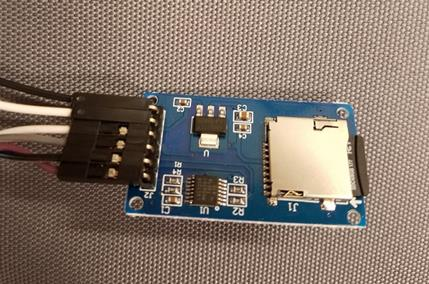
\includegraphics[width=3.614in,height=%
2.3981in]{PH4CAU00}
\end{figure}And we will need to wire this to
our Arduino. There are six pins on our SD card reader board. Those six pins
need to be wired to the following Arduino pins:

\begin{equation*}
\begin{tabular}{ll}
SD Card Reader & Arduino \\ 
GND & GND \\ 
VCC & +5V \\ 
MISO & Pin 12 \\ 
MOSI & Pin 11 \\ 
SCK & Pin 13 \\ 
CS & Pin 10%
\end{tabular}%
\end{equation*}

The pin names on the SD card reader board are usually on the back of the
card.\begin{figure}[h!]
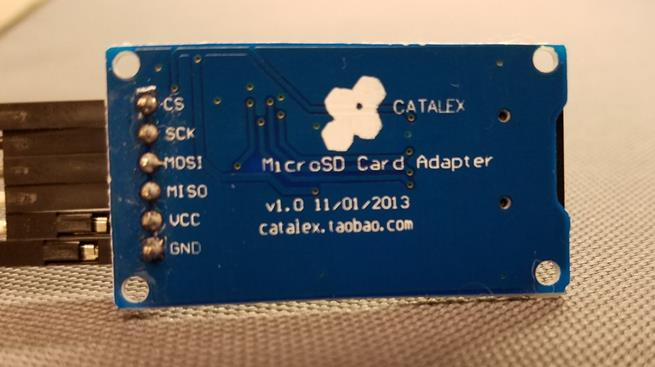
\includegraphics[width=4.5152in,height=2.5365in]{PH4CAV2N}
\end{figure}Of course, we will need a sketch
to tell the Arduino what to do with this new hardware. Here is an example:
\begin{verbatim}
////////////////////////////////////////////////////////////////////////////
//  SD card datalogger
//
// This example shows how to log data from three analog sensors
// to an SD card using the SD library.
//
// The circuit:
// * analog sensors on analog pin 0
// * SD card attached to SPI bus as follows:
// * MOSI - pin 11
// * MISO - pin 12
// * CLK  - pin 13
// * CS   - pin 10 (This one we can choose. Pin 10 is convenient
//                  but we could choose any of the digital pins)
// created  24 Nov 2010  by Tom Igoe
// modified 9 Apr 2012  by Tom Igoe
// Modified 26 Apr 2017 by Todd Lines
//
// This example code is in the public domain.
////////////////////////////////////////////////////////////////////////////
 
#include <SPI.h>
#include <SD.h>
 
const int CS_Pin = 10;       // this sets the pin for the CS connection
                             // to the SD card reader
 
////////////////////////////////////////////////////////////////////////////
void setup() {
    // Open serial communications and wait for port to open:
    Serial.begin(9600);    // the 9600 tells our Arduino how fast to send data
 
    // Check to see if the serial port is working
    while (!Serial) {
        ; // wait for serial port to connect. 
          // If it is, just keep going (don't do anything)
    }
    // Send a message to the Serial Monitor telling us that we are starting
    //     to use the SD card.
    Serial.print("Initializing SD card...");
 
    // See if the card is present and can be initialized.
    //    If there is a problem, tell us using the serial monitor.
    if (!SD.begin(CS_Pin)) {
        Serial.println("Card failed, or not present");
        // it didn't start the SD card write, so don't do anything more:
        return;
    }
    // But if the SD card did initialize, tell us on the serial monitor.
    Serial.println("card initialized.");
}
 
////////////////////////////////////////////////////////////////////////////
void loop() {
    // We will have to turn our voltage numbers into text to send to our file
    // let's make a text variable (called a string) for this
    String dataString = ""; 
 
    // let's choose our analog input  0 to read
    int analogPin = 0;
 
    // read the analog input
    int sensor = analogRead(analogPin);
 
    // make it text
    dataString += String(sensor);
  
    // open the file. note that only one file can be open at a time,
    // so you have to close this one before opening another.
    File dataFile = SD.open("datalog.txt", FILE_WRITE);
 
    // If the file is available, write to it, but then close it 
    //   right after. We will only keep the file open while we are 
    //   writing to it. This is safer. It helps prevent getting files 
    //   corrupted, and let's the Arduino keep adding to the file after 
    //   a problem.
    if (dataFile) {
        // print our data point
        dataFile.println(dataString);
 
        // close the file for safety
        dataFile.close();
 
        // print to the serial monitor too:
        Serial.println(dataString);
    }
 
    // if the file isn't open, pop up an error:
    else {
        Serial.println("error opening datalog.txt");
    }
}
////////////////////////////////////////////////////////////////////////////
////////////////////////////////////////////////////////////////////////////
\end{verbatim}

Make sure you understand each line of this code. It is a little fancy in
that it tries to check to make sure the SD card file is working properly and
warns you if something is wrong. But most of the code is comments. So don't
be discouraged by the length.

\section{Lab Assignment}

\begin{enumerate}
\item Finish any part of the last lab that you haven't done.

\item Using Python, Save Arduino data to a file on your computer

\begin{enumerate}
\item Wire up a simple voltmeter and load its sketch. Build a simple circuit
to test like we did back in section (\ref{Voltage Measurement with Meter}).
Start your Arduino and check to make sure voltages are going to the serial
port by looking at the serial monitor or plotter.

\item Check with your group members to make sure their simple voltmeters are
working. Help if they are not.

\item Start your Python system (Spyder or Canopy if you are following the
instructions given above) and write the program to read the serial port and
save the data to a file.

\item Close the serial monitor and/or serial plotter. Then run your Python
code. Check to make sure that the file of data is written properly. The
voltages written in the file should match what your power supply and circuit
provided.

\item Make sure you save this program and record what you did in your lab
notebook.

\item Make sure your lab group members all have Python programs that run and
save data correctly. Help if they do not.
\end{enumerate}

\item Together with your group, fill out a \textquotedblleft brainstorming
sheet\textquotedblright\ in preparation for your design project later in the
semester.

\item If there is time...add an SD card reader to your Arduino setup.

\begin{enumerate}
\item Wire up an SD card reader

\item Write the new sketch. The instructions given above should help.

\item Record data from your Arduino like a simple voltmeter.

\item Check to see if the SD card file has the voltages you expected.

\item Make sure you save your new sketch and record what you did in your lab
notebook.
\end{enumerate}
\end{enumerate}